\documentclass[journal,12pt,twocolumn]{IEEEtran}
%
\usepackage{setspace}
\usepackage{gensymb}
%\doublespacing
\singlespacing

%\usepackage{graphicx}
%\usepackage{amssymb}
%\usepackage{relsize}
\usepackage[cmex10]{amsmath}
%\usepackage{amsthm}
%\interdisplaylinepenalty=2500
%\savesymbol{iint}
%\usepackage{txfonts}
%\restoresymbol{TXF}{iint}
%\usepackage{wasysym}
\usepackage{amsthm}
%\usepackage{iithtlc}
\usepackage{mathrsfs}
\usepackage{txfonts}
\usepackage{stfloats}
\usepackage{bm}
\usepackage{cite}
\usepackage{cases}
\usepackage{subfig}
%\usepackage{xtab}
\usepackage{longtable}
\usepackage{multirow}
%\usepackage{algorithm}
%\usepackage{algpseudocode}
\usepackage{enumitem}
\usepackage{mathtools}
\usepackage{steinmetz}
\usepackage{tikz}
\usepackage{circuitikz}
\usepackage{verbatim}
\usepackage{tfrupee}
\usepackage[breaklinks=true]{hyperref}
%\usepackage{stmaryrd}
\usepackage{tkz-euclide} % loads  TikZ and tkz-base
\usetkzobj{all}
\usetikzlibrary{decorations.markings}
\usetikzlibrary{shapes.geometric}
\newif\iflabrev
\usepackage{listings}
    \usepackage{color}                                            %%
    \usepackage{array}                                            %%
    \usepackage{longtable}                                        %%
    \usepackage{calc}                                             %%
    \usepackage{multirow}                                         %%
    \usepackage{hhline}                                           %%
    \usepackage{ifthen}                                           %%
  %optionally (for landscape tables embedded in another document): %%
    \usepackage{lscape}     
\usepackage{multicol}
\usepackage{chngcntr}
%\usepackage{enumerate}

%\usepackage{wasysym}
%\newcounter{MYtempeqncnt}
\DeclareMathOperator*{\Res}{Res}
%\renewcommand{\baselinestretch}{2}
\renewcommand\thesection{\arabic{section}}
\renewcommand\thesubsection{\thesection.\arabic{subsection}}
\renewcommand\thesubsubsection{\thesubsection.\arabic{subsubsection}}

\renewcommand\thesectiondis{\arabic{section}}
\renewcommand\thesubsectiondis{\thesectiondis.\arabic{subsection}}
\renewcommand\thesubsubsectiondis{\thesubsectiondis.\arabic{subsubsection}}

% correct bad hyphenation here
\hyphenation{op-tical net-works semi-conduc-tor}
\def\inputGnumericTable{}                                 %%

\lstset{
%language=C,
frame=single, 
breaklines=true,
columns=fullflexible
}
%\lstset{
%language=tex,
%frame=single, 
%breaklines=true
%}

\begin{document}
%


\newtheorem{theorem}{Theorem}[section]
\newtheorem{problem}{Problem}
\newtheorem{proposition}{Proposition}[section]
\newtheorem{lemma}{Lemma}[section]
\newtheorem{corollary}[theorem]{Corollary}
\newtheorem{example}{Example}[section]
\newtheorem{definition}[problem]{Definition}
%\newtheorem{thm}{Theorem}[section] 
%\newtheorem{defn}[thm]{Definition}
%\newtheorem{algorithm}{Algorithm}[section]
%\newtheorem{cor}{Corollary}
\newcommand{\BEQA}{\begin{eqnarray}}
\newcommand{\EEQA}{\end{eqnarray}}
\newcommand{\define}{\stackrel{\triangle}{=}}
\bibliographystyle{IEEEtran}
%\bibliographystyle{ieeetr}
\providecommand{\mbf}{\mathbf}
\providecommand{\pr}[1]{\ensuremath{\Pr\left(#1\right)}}
\providecommand{\qfunc}[1]{\ensuremath{Q\left(#1\right)}}
\providecommand{\sbrak}[1]{\ensuremath{{}\left[#1\right]}}
\providecommand{\lsbrak}[1]{\ensuremath{{}\left[#1\right.}}
\providecommand{\rsbrak}[1]{\ensuremath{{}\left.#1\right]}}
\providecommand{\brak}[1]{\ensuremath{\left(#1\right)}}
\providecommand{\lbrak}[1]{\ensuremath{\left(#1\right.}}
\providecommand{\rbrak}[1]{\ensuremath{\left.#1\right)}}
\providecommand{\cbrak}[1]{\ensuremath{\left\{#1\right\}}}
\providecommand{\lcbrak}[1]{\ensuremath{\left\{#1\right.}}
\providecommand{\rcbrak}[1]{\ensuremath{\left.#1\right\}}}
\theoremstyle{remark}
\newtheorem{rem}{Remark}
\newcommand{\sgn}{\mathop{\mathrm{sgn}}}
\providecommand{\abs}[1]{\left\vert#1\right\vert}
\providecommand{\res}[1]{\Res\displaylimits_{#1}} 
\providecommand{\norm}[1]{\left\lVert#1\right\rVert}
%\providecommand{\norm}[1]{\lVert#1\rVert}
\providecommand{\mtx}[1]{\mathbf{#1}}
\providecommand{\mean}[1]{E\left[ #1 \right]}
\providecommand{\fourier}{\overset{\mathcal{F}}{ \rightleftharpoons}}
%\providecommand{\hilbert}{\overset{\mathcal{H}}{ \rightleftharpoons}}
\providecommand{\system}{\overset{\mathcal{H}}{ \longleftrightarrow}}
	%\newcommand{\solution}[2]{\textbf{Solution:}{#1}}
\newcommand{\solution}{\noindent \textbf{Solution: }}
\newcommand{\cosec}{\,\text{cosec}\,}
\providecommand{\dec}[2]{\ensuremath{\overset{#1}{\underset{#2}{\gtrless}}}}
\newcommand{\myvec}[1]{\ensuremath{\begin{pmatrix}#1\end{pmatrix}}}
\newcommand{\mydet}[1]{\ensuremath{\begin{vmatrix}#1\end{vmatrix}}}
%\numberwithin{equation}{section}
\numberwithin{equation}{subsection}
%\numberwithin{problem}{section}
%\numberwithin{definition}{section}
\makeatletter
\@addtoreset{figure}{problem}
\makeatother
\let\StandardTheFigure\thefigure
\let\vec\mathbf
%\renewcommand{\thefigure}{\theproblem.\arabic{figure}}
\renewcommand{\thefigure}{\theproblem}
%\setlist[enumerate,1]{before=\renewcommand\theequation{\theenumi.\arabic{equation}}
%\counterwithin{equation}{enumi}
%\renewcommand{\theequation}{\arabic{subsection}.\arabic{equation}}
\def\putbox#1#2#3{\makebox[0in][l]{\makebox[#1][l]{}\raisebox{\baselineskip}[0in][0in]{\raisebox{#2}[0in][0in]{#3}}}}
     \def\rightbox#1{\makebox[0in][r]{#1}}
     \def\centbox#1{\makebox[0in]{#1}}
     \def\topbox#1{\raisebox{-\baselineskip}[0in][0in]{#1}}
     \def\midbox#1{\raisebox{-0.5\baselineskip}[0in][0in]{#1}}
\vspace{3cm}
\title{
%	\logo{
Control Systems
%	}
}
\author{ G V V Sharma$^{*}$% <-this % stops a space
	\thanks{*The author is with the Department
		of Electrical Engineering, Indian Institute of Technology, Hyderabad
		502285 India e-mail:  gadepall@iith.ac.in. All content in this manual is released under GNU GPL.  Free and open source.}
	
}	
%\title{
%	\logo{Matrix Analysis through Octave}{\begin{center}\includegraphics[scale=.24]{tlc}\end{center}}{}{HAMDSP}
%}
% paper title
% can use linebreaks \\ within to get better formatting as desired
%\title{Matrix Analysis through Octave}
%
%
% author names and IEEE memberships
% note positions of commas and nonbreaking spaces ( ~ ) LaTeX will not break
% a structure at a ~ so this keeps an author's name from being broken across
% two lines.
% use \thanks{} to gain access to the first footnote area
% a separate \thanks must be used for each paragraph as LaTeX2e's \thanks
% was not built to handle multiple paragraphs
%
%\author{<-this % stops a space
%\thanks{}}
%}
% note the % following the last \IEEEmembership and also \thanks - 
% these prevent an unwanted space from occurring between the last author name
% and the end of the author line. i.e., if you had this:
% 
% \author{....lastname \thanks{...} \thanks{...} }
%                     ^------------^------------^----Do not want these spaces!
%
% a space would be appended to the last name and could cause every name on that
% line to be shifted left slightly. This is one of those "LaTeX things". For
% instance, "\textbf{A} \textbf{B}" will typeset as "A B" not "AB". To get
% "AB" then you have to do: "\textbf{A}\textbf{B}"
% \thanks is no different in this regard, so shield the last } of each \thanks
% that ends a line with a % and do not let a space in before the next \thanks.
% Spaces after \IEEEmembership other than the last one are OK (and needed) as
% you are supposed to have spaces between the names. For what it is worth,
% this is a minor point as most people would not even notice if the said evil
% space somehow managed to creep in.
% The paper headers
%\markboth{Journal of \LaTeX\ Class Files,~Vol.~6, No.~1, January~2007}%
%{Shell \MakeLowercase{\textit{et al.}}: Bare Demo of IEEEtran.cls for Journals}
% The only time the second header will appear is for the odd numbered pages
% after the title page when using the twoside option.
% 
% *** Note that you probably will NOT want to include the author's ***
% *** name in the headers of peer review papers.                   ***
% You can use \ifCLASSOPTIONpeerreview for conditional compilation here if
% you desire.
% If you want to put a publisher's ID mark on the page you can do it like
% this:
%\IEEEpubid{0000--0000/00\$00.00~\copyright~2007 IEEE}
% Remember, if you use this you must call \IEEEpubidadjcol in the second
% column for its text to clear the IEEEpubid mark.
% make the title area
\maketitle
\newpage
\tableofcontents
\bigskip
\renewcommand{\thefigure}{\theenumi}
\renewcommand{\thetable}{\theenumi}
%\renewcommand{\theequation}{\theenumi}
%\begin{abstract}
%%\boldmath
%In this letter, an algorithm for evaluating the exact analytical bit error rate  (BER)  for the piecewise linear (PL) combiner for  multiple relays is presented. Previous results were available only for upto three relays. The algorithm is unique in the sense that  the actual mathematical expressions, that are prohibitively large, need not be explicitly obtained. The diversity gain due to multiple relays is shown through plots of the analytical BER, well supported by simulations. 
%
%\end{abstract}
% IEEEtran.cls defaults to using nonbold math in the Abstract.
% This preserves the distinction between vectors and scalars. However,
% if the journal you are submitting to favors bold math in the abstract,
% then you can use LaTeX's standard command \boldmath at the very start
% of the abstract to achieve this. Many IEEE journals frown on math
% in the abstract anyway.
% Note that keywords are not normally used for peerreview papers.
%\begin{IEEEkeywords}
%Cooperative diversity, decode and forward, piecewise linear
%\end{IEEEkeywords}
% For peer review papers, you can put extra information on the cover
% page as needed:
% \ifCLASSOPTIONpeerreview
% \begin{center} \bfseries EDICS Category: 3-BBND \end{center}
% \fi
%
% For peerreview papers, this IEEEtran command inserts a page break and
% creates the second title. It will be ignored for other modes.
%\IEEEpeerreviewmaketitle
\begin{abstract}
This manual is an introduction to control systems based on GATE problems.Links to sample Python codes are available in the text.  
\end{abstract}
Download python codes using 
\begin{lstlisting}
svn co https://github.com/gadepall/school/trunk/control/codes
\end{lstlisting}
\section{Circuit Design}
\begin{enumerate}[label=\thesubsection.\arabic*.,ref=\thesubsection.\theenumi]
\numberwithin{equation}{enumi}

\item For the feedback current amplifier shown in \ref{fig:Input}, Draw the Small-Signal Model.eglect the Early effect in $Q_{1}$ and $Q_{2}$.\\
\begin{figure}[h!]
	\begin{center}
		\resizebox{\columnwidth/1}{!}{\begin{circuitikz}[american]
\ctikzset{tripoles/mos style/arrows}
\draw  (0,0) node[ground](GND){} -- (0,1) to[isource, l= $I_{s}$] (0,3) -- (2,3) to[R=$R_{F}$, i=$I_{f}$] (4,3) -- (6,3)node[label={right:C}]{} to[R=$R_{m}$] (6,0) node[ground](GND){} (6,0);

\draw (1,5) node[nmos,](Q1){};
\draw (1,3) node[label={below:A}]{} to[short,i=$I_{i}$] (Q1.S);
\draw (Q1.center) node[right]{{$Q_{1}$}};
\draw (Q1.G) -- (0,5) node[ground](GND){};
\draw (1,9) node[vcc](VCC){$V_{CC}$} (1,9);
\draw  (1,6)node[label={left:B}]{} -- (1,6.5) to[R=$R_{D}$, i=$I_{i}$] (1,9);
\draw (Q1.D) -- (1,6);

\draw (6,6)node[pmos,](Q2){};
\draw (Q2.D) to[R=$R_{L}$,i=$I_{o}$] (6,3);
\draw (Q2.center) node[right]{{$Q_{2}$}};
\draw (Q2.G) -- (1,6);
\draw (Q2.S) -- (6,9) node[vcc](VCC){$V_{CC}$} (6,10);
\end{circuitikz}
}
	\end{center}
	\caption{}
	\label{fig:Input}
\end{figure}

\solution
While drawing a Small-Signal Model, we ground all constant voltage sources and open all constant current sources. All Small-Signal paramters are obtained from DC-Analysis of the circuit. Neglecting Early effect, in Small-Signal Analysis a N-MOSFET is modelled as a Current Source with value of current equal to $g_{m}v_{gs}$ flowing from Drain to Source. Whereas a P-MOSFET is modelled as a Current Source with value of current equal to $g_{m}v_{sg}$ flowing from Source to Drain.
\begin{figure}[h!]
	\begin{center}
		\resizebox{\columnwidth/1}{!}{\begin{circuitikz}[american]
\ctikzset{tripoles/mos style/arrows}
\draw  (0,0) node[ground](GND){} -- (0,1) to[isource, l= $I_{s}$] (0,3) -- (2,3) to[R=$R_{F}$, i=$I_{f}$] (4,3) -- (6,3)node[label={right:C}]{} to[R=$R_{m}$] (6,0) node[ground](GND){} (6,0);

\draw (1,3) node[label={below:A}]{} to[short,i=$I_{i}$] (1,4);
\draw (1,6) node[label={right:B}]{} to[cisource, l= $-g_{m_{1}}v_{A}$] (1,4);
\draw (1,4) to[short, -o] (-1,4) node[label={above:$-$}]{} node[label={below:$S_{1}$}]{};
\draw (-1,5.5) node[label={below:$-v_{A}$}]{};
\draw (-2,6) node[label={below:$G_{1}$}]{} to[short, -o] (-1,6) node[label={below:$+$}]{};
\draw (1,6) to[R=$R_{D}$, i=$I_{i}$] (1,9);
\draw (1,9) node[ground,rotate=180](GND){} (1,9);

\draw (6,7) to[R=$R_{L}$,i=$I_{o}$] (6,3);
\draw (6,8) to[cisource, l= $-g_{m_{2}}v_{B}$] (6,7);
\draw (6,6.5) to[short, -o] (4,6.5) node[label={above:$-$}]{} node[label={below:$G_{2}$}]{};
\draw (4,8) node[label={below:$-v_{B}$}]{};
\draw (3,8.5) node[label={below:$S_{2}$}]{} to[short, -o] (4,8.5) node[label={below:$+$}]{};
\draw (6,7) -- (6,9);
\draw (6,9) node[ground,rotate=180](GND){} (6,9);

\end{circuitikz}
}
	\end{center}
	\caption{Small Signal Model}
	\label{fig:Small_Signal}
\end{figure}

%------------------------------------------------------------------------%

\item Describe how the given circuit is a Negetive Feedback Current Amplifier.\\
\solution 
For the feedback to be negative, $I_{f}$ must have the same polarity as $I_{s}$. To ascertain that this is the case, we assume an increase in $I_{s}$ and follow the change around the loop: An increase in $I_{s}$ causes $I_{i}$ to increase and the drain voltage of $Q_{1}$ will increase. Since this voltage is applied to the gate of the p-channel device $Q_{2}$ , its increase will cause $I_{o}$ , the drain current of $Q_{2}$, to decrease. Thus, the voltage across $R_{M}$ will decrease, which will cause $I_{f}$ to increase. This is the same polarity assumed for the initial change in
$I_{s}$, verifying that the feedback is indeed negative.
%------------------------------------------------------------------------%

\item Find the Expression for the Open-Loop Gain $G=\frac{I_{o}}{I_{i}}$, from the Small-Signal Model. For simplicity, neglect the Early effect in $Q_{1}$ and $Q_{2}$.\\
\solution
In Small-Signal Model,
\begin{align}
v_{B} = I_{i}R_{D}\\
v_{gs_{2}} = v_{B} = I_{i}R_{D}
\end{align}

In Small-Signal Analysis, P-MOSFET is modelled as a current source where current flows from Source to Drain. So, the value of current flowing from Source to Drain in P-MOSFET is,
\begin{align}
I_{o} =  -g_{m_{2}}v_{gs_{2}} = -g_{m_{2}}I_{i}R_{D}
\end{align}
So, the Open-Circuit Gain is
\begin{align}
G = \frac{I_{o}}{I_{i}} =  -g_{m_{2}}R_{D}
\end{align}
%------------------------------------------------------------------------%

\item Find the Expression of the Feedback Factor $H = \frac{I_{f}}{I_{o}}$, from Small-Signal Model. For simplicity, neglect the Early effect in $Q_{1}$ and $Q_{2}$.\\
\solution\\
$I_{o}$ is fed to a current divider formed by $R_{M}$ and $R_{F}$. Current Mixing results in a reduced input resistance, the voltage at the source node of $Q_{2}$ will be close to zero. Hence the voltage at point 'A' is very small and is considered, $v_{A} \simeq 0$. So $R_{F}$ and $R_{M}$ are parallel and Voltage Drop across them is same.
\begin{align}
(I_{o} + I_{f})R_{M} \simeq -I_{f}R_{F}\\
\frac{I_{f}}{I_{o}} \simeq -\frac{R_{M}}{R_{F}+R_{M}}
\end{align}
So, the Feedback Factor,
\begin{align}
H \equiv \frac{I_{f}}{I_{o}} \simeq-\frac{R_{M}}{R_{F}+R_{M}}
\end{align}
%------------------------------------------------------------------------%
\item Find the Expression for the Closed-Loop Gain $T=\frac{I_{o}}{I_{s}}$. For simplicity, neglect the Early effect in $Q_{1}$ and $Q_{2}$.\\
\solution \\
From Open-Loop Gain and Feedback Factor,
\begin{align}
I_{s} = I_{i} + I_{f}\\
I_{s} = \frac{I_{o}}{G} + H I_{o}\\
GI_{s} = I_{o}(1+GH)\\
\frac{I_{o}}{I_{s}} = \frac{G}{1+GH}\\
\frac{I_{o}}{I_{s}}=-\frac{g_{m_{2}} R_{D}}{1+g_{m_{2}} R_{D} /\left(1+\frac{R_{F}}{R_{M}}\right)}
\end{align}

So the Block Diagram of Feedback Current Amplifier is
\begin{figure}[ht!]
	\begin{center}
		\resizebox{\columnwidth}{!}{\begin{circuitikz}[american]

\draw (2,2)  node[op amp] (OA) {};
\draw (OA.up) -- ++(0, 0.3) node[vcc]{$+10V$};
\draw (OA.down) -- ++(0,-0.3) node[vee]{$-10V$};
\draw (OA.+) -- (0,1.5) to[vsourcesin, l= $v_{s}$] (0,0) node[ground](GND){};
\draw (OA.-) -- (0,2.5) node[ground, rotate=270](GND){};
\draw (OA.out) -- (3,2) node[label={above:$v_{a}$}]{};
\draw (3,2) to[R=$R_{1}$] (5.5,2) node[label={above:$v_{b}$}]{} to[C,l_=$C_{1}$] (5.5,0) node[ground](GND){};

\draw (7.5,2.5) node[op amp] (OB) {};
\draw (OB.up) -- ++(0, 0.3) node[vcc]{$+10V$};
\draw (OB.down) -- ++(0,-0.3) node[vee]{$-10V$};
\draw (OB.+) -- (5.5,2);
\draw (OB.-) -- ++(-0.5,0) node[ground,rotate=270](GND){};;
\draw (OB.out) to[R=$R_{2}$] (10.5,2.5) node[label={above:$v_{c}$}]{} to[C,l_=$C_{2}$] (10.5,0) node[ground](GND){};

\draw (12.5,3) node[op amp] (OC) {};
\draw (OC.up) -- ++(0, 0.3) node[vcc]{$+10V$};
\draw (OC.down) -- ++(0,-0.3) node[vee]{$-10V$};
\draw (OC.+) -- (10.5,2.5);
\draw (OC.-) -- ++(-0.5,0) node[ground,rotate=270](GND){};;
\draw (OC.out) to[R=$R_{3}$] (15.5,3) node[label={right:$v_{o}$}]{} to[C,l_=$C_{3}$] (15.5,0) node[ground](GND){};

\end{circuitikz}
}
	\end{center}
	\caption{}
	\label{fig:Control_System}
\end{figure}

where $G = -g_{m_{2}} R_{D}$ and $H = -\frac{R_{M}}{R_{F}+R_{M}}$\\

So, the value of Closed-Loop Gain is
\begin{align}
T = \frac{I_{o}}{I_{s}}=-\frac{g_{m_{2}} R_{D}}{1+g_{m_{2}} R_{D} /\left(1+\frac{R_{F}}{R_{M}}\right)}
\end{align}
%------------------------------------------------------------------------%

\end{enumerate}

\section{Assignment}
%\begin{enumerate}[label=\arabic*.,ref=\theenumi]
\begin{enumerate}[label=\thesection.\arabic*.,ref=\thesection.\theenumi]
\numberwithin{equation}{enumi}
%-------------------------------------------------------------------------------------------------%
%2.1.6
\item Find the frequency for which $PM = 90 \degree$.  Assume $H$ to be constant.
\\
%\solution Letting 
%\item Find the frequencies for which phase margins are $90\degree$ and $45\degree$ respectively?\\
\solution $\because \phase{H\brak{f}} = 1$, 
\begin{align}
\phase{G\brak{f_{90}}H\brak{f_{90}}} &= \phase{G\brak{f_{90}}} = 90\degree - 180\degree
\\
&= -90\degree
\label{eq:ee18btech11014_Gpm90}
%\\
%\implies \abs{G\brak{f_{90}}H\brak{f_{90}}} &=1
\end{align}
%
%From \eqref{eq:ee18btech11014_G_ang},
%%
%\begin{multline}
%\phi\brak{f} =
%\\
%-\sbrak{\tan ^{-1}\brak{\frac{f}{10^{5}}}+\tan ^{-1}\brak{\frac{f}{10^{6}}}+\tan ^{-1}\brak{\frac{f}{10^{7}}}}
%\end{multline}
The Bode plot in Fig. 	\ref{fig:ee18btech11014_Bode} shows that 
\begin{align}
\abs{G(f)} < 1, \quad f > 10^8
\end{align}
%
Also, 
\begin{align}
\tan^{-1}\brak{\frac{f}{10^{7}}} \approx 0, \quad f < 10^8
\end{align}

Thus, from  \eqref{eq:ee18btech11014_G_ang} and \eqref{eq:ee18btech11014_Gpm90},
%
\begin{align}
\phi\brak{f} &\approx
-\sbrak{\tan ^{-1}\brak{\frac{f}{10^{5}}}+\tan ^{-1}\brak{\frac{f}{10^{6}}}}
\\
&= -90 \degree
\\
\implies f_{90} &= 3.162 \times 10^{5}
\end{align}
after simplification.
%-------------------------------------------------------------------------------------------------%
\item Find $H$ when the $PM = 90 \degree$.
\\
\solution By definition of the PM, 
\begin{align}
\abs{G\brak{f_{90}}H\brak{f_{90}}} &=1
\\
\implies \abs{H\brak{f_{90}}} &=\frac{1}{\abs{G\brak{f_{90}}}}
\label{eq:ee18btech11014_GH_PM_90}
\end{align}
%
From \eqref{eq:ee18btech11014_G_piece},
\begin{align}
20 \log \abs{G(f)} &= 200 - 20\log(3.162 \times 10^{5})\\
&= 90 dB \\
\implies \abs{G(f)} &= 3.1625 \times 10^{4}
\\
\implies H &= 3.162 \times 10^{-5}
\end{align}
using \eqref{eq:ee18btech11014_GH_PM_90}.
%-------------------------------------------------------------------------------------------------%
\item Design the closed loop circuit for $PM = 90 \degree$
\\
\solution See Fig. 	\ref{fig:ee18btech11014_Closed-Loop Circuit alpha=90}, where Fig. 	\ref{fig:ee18btech11014_Feedback Circuit} is used for the feedback $H$ with $R_M = 0.3162 M \ohm$ and 	$R_F = 10 \ohm$.

\begin{figure}[ht!]
	\begin{center}
		\resizebox{\columnwidth}{!}{\begin{circuitikz}[american]

\draw (2,2)  node[op amp] (OA) {};
\draw (OA.up) -- ++(0, 0.3) node[vcc]{$+10V$};
\draw (OA.down) -- ++(0,-0.3) node[vee]{$-10V$};
\draw (OA.+) -- (0,1.5) to[vsourcesin, l= $v_{s}$] (0,0) node[ground](GND){};
\draw (OA.-) -- (0,2.5) to[R=$10\ohm$] (-2,2.5) node[ground, rotate=270](GND){};
\draw (OA.out) -- (3,2) node[label={below:$v_{a}$}]{};
\draw (3,2) to[R=$10^{2}\ohm$] (5.5,2) node[label={above:$v_{b}$}]{} to[C,l_=$\frac{10^{-9}}{2\pi}F$] (5.5,0) node[ground](GND){};
\draw (5.5,2) to[R=$10^{3}\ohm$] (8,2) node[label={above:$v_{c}$}]{} to[C,l_=$\frac{10^{-9}}{2\pi}F$] (8,0) node[ground](GND){};
\draw (8,2) to[R=$10^{4}\ohm$] (10.5,2) to[C,l_=$\frac{10^{-9}}{2\pi}F$] (10.5,0) node[ground](GND){};
\draw (10.5,2) -- (11.5,2) node[label={above:$v_{o}$}]{};
\draw (10.5,2) -- (10.5,4) to[R=$3.162\times 10^{5}\ohm$] (0,4) -- (0,2.5);

\end{circuitikz}
}
	\end{center}
	\caption{}
	\label{fig:ee18btech11014_Closed-Loop Circuit alpha=90}
\end{figure}
%-------------------------------------------------------------------------------------------------%

\item Using ngspice, find the output of the \ref{fig:ee18btech11014_Closed-Loop Circuit alpha=90} for Unit-Step Signal and Sinusoidal Signal as Input.\\
\solution\\
Check the following spice file for circuits for inputs Unit-Step and Sinusoidal Signal respectively.
\begin{lstlisting}
spice/ee18btech11014/ee18btech11014_1.net
spice/ee18btech11014/ee18btech11014_2.net
\end{lstlisting}

Run the following Python Code for Visualising the Responses for Inputs.
\begin{lstlisting}
spice/ee18btech11014/EE18BTECH11014_Simulation-1,2.py
\end{lstlisting}

The Responses are shown in Fig.\ref{fig:PM=90}
\begin{figure}[ht!]
	\begin{center}
		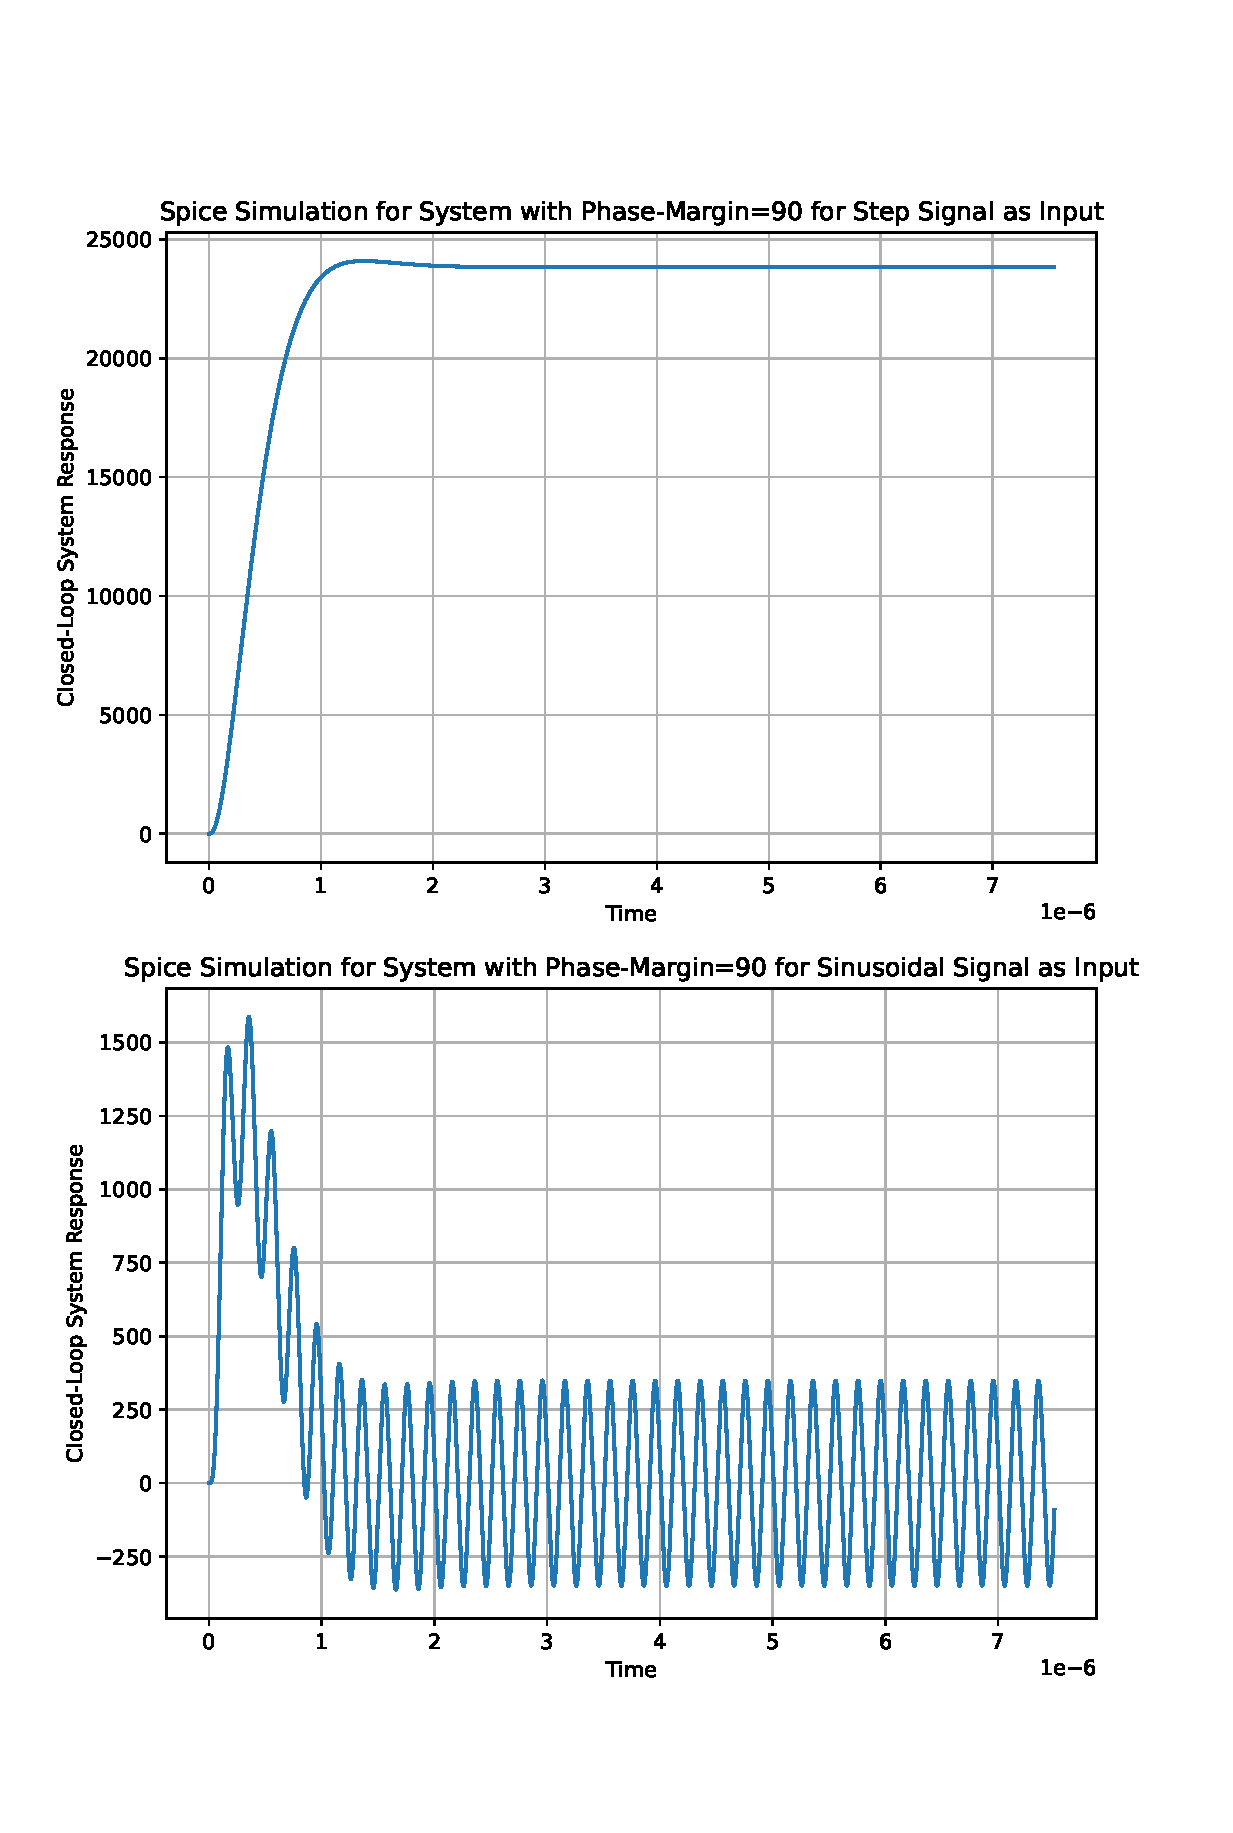
\includegraphics[width=\columnwidth]{./figs/ee18btech11014/ee18btech11014_Spice_Result_PM=90.eps}
	\end{center}
	\caption{}
	\label{fig:PM=90}
\end{figure}
%-------------------------------------------------------------------------------------------------%
\item Repeat all the above for $PM = 45\degree$.
%-------------------------------------------------------------------------------------------------%

%-\tan^{-1}\left(f/10^{5}\right)-\tan^{-1}\left(f/10^{6}\right) = -90\\
%\tan^{-1}\left(f/10^{5}\right)+\tan^{-1}\left(f/10^{6}\right) = 90\\
%\tan^{-1}\left(f/10^{5}\right) = 90-\tan^{-1}\left(f/10^{6}\right)\\
%\tan^{-1}\left(f/10^{5}\right) = \cot^{-1}\left(f/10^{6}\right)\\
%\tan^{-1}\left(f/10^{5}\right) = \tan^{-1}\left(10^{6}/f\right)\\
%f^{2} = 10^{11}\\
%f = 3.162 \times 10^{5}
%\end{align}
%
%So, the approximate value of $f$ at which Phase Margin is $90\degree$ is $f=3.162 \times 10^{5} Hz$.\\

%Similarly let Phase Margin be $\alpha = 45\degree$. Then,
%\begin{align}
%\alpha = \phi - (-180\degree)\\
%\phi = -180\degree + \alpha\\
%\phi = -135\degree
%\end{align}
%
%So, by the definition of Phase-Margin, at $\phi = -135\degree$ , $|GH| = 1 $.  The value of $\phi = -135\degree$ aproximately at poles $f=10^{6} Hz$. 
%
%So, the approximate value of $f$ at which Phase Margin is $45\degree$ is $f=10^{6}$.\\
%%-------------------------------------------------------------------------------------------------%
%%2.1.7
%\item Find the minimum values of Closed-Loop Voltage Gain for which phase margins are $90\degree$ and  $45\degree$ respectively\\
%\solution\\
%For $\alpha=90\degree$,
%\begin{align}
%f=3.162 \times 10^{5}
%\end{align}
%By substituting $f$ in Open-Loop Gain $G(f)$ (assuming poles are far part), 
%\begin{align}
%G(f) = 200 - 20log(3.162 \times 10^{5})\\
%G(f) = 90 dB \\
%G = 3.1625 \times 10^{4}
%\end{align}
%
%At that $f=3.162 \times 10^{5}$, 
%\begin{align}
%H = \frac{1}{G}\\
%H = 3.162 \times 10^{-5}
%\end{align}
%
%The minimum value of Closed-Loop Gain occurs at $|GH| \gg 1$ and the value of Closed-Loop Gain is $T=\frac{1}{H}$
%
%\begin{align}
%T = \frac{1}{H} = 3.1625 \times 10^{4}
%\end{align}
%
%\textbf{So, The minimum value of Closed-Loop Gain with Phase Margin equal to $\alpha=90\degree$ is $T_{min} = 3.1625 \times 10^{4}$.}\\
%
%For $\alpha=45\degree$,
%\begin{align}
%f=10^{6}
%\end{align}
%By substituting $f$ in Open-Loop Gain $G(f)$ (assuming poles are far part), 
%\begin{align}
%G(f) = 200 - 20log(10^{6})\\
%G(f) = 80 dB \\
%G = 10^{4}
%\end{align}
%
%At that $f = 10^{6}$, 
%\begin{align}
%H = \frac{1}{G}\\
%H = 10^{-4}
%\end{align}
%
%The minimum value of Closed-Loop Gain occurs at $|GH| \gg 1$ and the value of Closed-Loop Gain is $T=\frac{1}{H}$
%
%\begin{align}
%T = \frac{1}{H} = 10^{4}
%\end{align}
%
%\textbf{So, The minimum value of Closed-Loop Gain with Phase Margin equal to $\alpha=45\degree$ is $T_{min} = 10^{4}$.}\\
%%-------------------------------------------------------------------------------------------------%
%
%\item Design a Feedback circuit for Phase Margin $\alpha=45^{\circ}$.\\
%\solution
%\begin{figure}[ht!]
%	\begin{center}
%		\resizebox{\columnwidth/2}{!}{\begin{circuitikz}[american]
\ctikzset{tripoles/mos style/arrows}
\draw (1,2) to[short, -o] (0,2) node[label={below:$v_{o}$}]{};
\draw (1,2) to[R=$100k\ohm$] (2,2) -- (3,2) to[R=$10\ohm$] (3,0) node[ground](GND){};
\draw (3,2) to[short, -o] (4,2) node[label={below:$v_{f}$}]{};
\end{circuitikz}
}
%	\end{center},
%	\caption{}
%	\label{fig:ee18btech11014_alpha=45}
%\end{figure}
%\begin{align}
%v_{f} = \frac{10}{10 + 10^{5}} \times v_{o}\\
%v_{f} \approx 10^{-4} v_{o}\\
%\frac{v_{f}}{v_{o}} \approx 10^{-4}\\
%H(s) = 10^{-4}
%\end{align}
%%-------------------------------------------------------------------------------------------------%
%
%\item Design a Feedback circuit for Phase Margin $\alpha=90^{\circ}$.\\
%\solution
%\begin{figure}[ht!]
%	\begin{center}
%		\resizebox{\columnwidth/2}{!}{\begin{circuitikz}[american]
\ctikzset{tripoles/mos style/arrows}
\draw (1,2) to[short, -o] (0,2) node[label={below:$v_{o}$}]{};
\draw (1,2) to[R=$0.3162 M\ohm$] (2,2) -- (3,2) to[R=$10\ohm$] (3,0) node[ground](GND){};
\draw (3,2) to[short, -o] (4,2) node[label={below:$v_{f}$}]{};
\end{circuitikz}
}
%	\end{center},
%	\caption{}
%	\label{fig:ee18btech11014_alpha=90}
%\end{figure}
%\begin{align}
%v_{f} = \frac{10}{10 + 3.162\times 10^{5}} \times v_{o}\\
%v_{f} \approx 3.162\times 10^{-5} v_{o}\\
%\frac{v_{f}}{v_{o}} \approx 3.162\times 10^{-5}\\
%H(s) = 3.162\times 10^{-5}
%\end{align}
%%-------------------------------------------------------------------------------------------------%
%
%\item  Design a Closed-Loop Transfer Function by combining both the Open-Loop and Feedback Circuits for phase Margin $\alpha=45^{\circ}$. Also draw its Equivalent Circuit\\
%\solution\\
%The Closed-Loop Circuit is
%\begin{figure}[ht!]
%	\begin{center}
%		\resizebox{\columnwidth}{!}{\begin{circuitikz}[american]

\draw (2,2)  node[op amp] (OA) {};
\draw (OA.up) -- ++(0, 0.3) node[vcc]{$+10V$};
\draw (OA.down) -- ++(0,-0.3) node[vee]{$-10V$};
\draw (OA.+) -- (0,1.5) to[vsourcesin, l= $v_{s}$] (0,0) node[ground](GND){};
\draw (OA.-) -- (0,2.5) to[R=$10\ohm$] (-2,2.5) node[ground, rotate=270](GND){};
\draw (OA.out) -- (3,2) node[label={below:$v_{a}$}]{};
\draw (3,2) to[R=$10^{2}\ohm$] (5.5,2) node[label={above:$v_{b}$}]{} to[C,l_=$\frac{10^{-9}}{2\pi}F$] (5.5,0) node[ground](GND){};
\draw (5.5,2) to[R=$10^{3}\ohm$] (8,2) node[label={above:$v_{c}$}]{} to[C,l_=$\frac{10^{-9}}{2\pi}F$] (8,0) node[ground](GND){};
\draw (8,2) to[R=$10^{4}\ohm$] (10.5,2) to[C,l_=$\frac{10^{-9}}{2\pi}F$] (10.5,0) node[ground](GND){};
\draw (10.5,2) -- (11.5,2) node[label={above:$v_{o}$}]{};
\draw (10.5,2) -- (10.5,4) to[R=$10^{5}\ohm$] (0,4) -- (0,2.5);

\end{circuitikz}
}
%	\end{center}
%	\caption{}
%	\label{fig:ee18btech11014_Closed-Loop Circuit alpha=45}
%\end{figure}
%
%The Equivalent Circuit of Closed-Loop Circuit is
%\begin{figure}[ht!]
%	\begin{center}
%		\resizebox{\columnwidth}{!}{\begin{circuitikz}[american]-1
\draw (-3,0) node[ground](GND){} to[vsourcesin, l= $v_{s}$] (-3,2) to[short,-o] (0.25,2) node[label={below:$+$}]{};
\draw (0,0.1) to[R=$10\ohm$,v=$v_{f}$] (-2,0.1) node[ground](GND){}; 
\draw (0,0.1) -- (1,0.1) -- (1,4) to[R=$10^{5}\ohm$] (10.5,4) -- (10.5,2);


\draw (0.25,0.1) to[short,-o] (0.25,0.1) node[label={above:$-$}]{};
\draw (0.25,0.625) node[label={$v_{i}$}] {};


\draw (3,2) node[label={above:$v_{a}$}]{};
\draw (3,0) node[ground](GND){} to[vsourcesin, l= $10^5 v_{i}$] (3,2);
\draw (3,2) to[R=$10^{2}\ohm$] (5.5,2) node[label={above:$v_{b}$}]{} to[C,l_=$\frac{10^{-9}}{2\pi}F$] (5.5,0) node[ground](GND){};
\draw (5.5,2) to[R=$10^{3}\ohm$] (8,2) node[label={above:$v_{c}$}]{} to[C,l_=$\frac{10^{-9}}{2\pi}F$] (8,0) node[ground](GND){};
\draw (8,2) to[R=$10^{4}\ohm$] (10.5,2) to[C,l_=$\frac{10^{-9}}{2\pi}F$] (10.5,0) node[ground](GND){};
\draw (10.5,2) -- (11.5,2) node[label={above:$v_{o}$}]{};

\end{circuitikz}
}
%	\end{center},
%	\caption{}
%	\label{fig:ee18btech11014_Closed-Loop Equivalent Circuit alpha=45}
%\end{figure}
%
%From the Equivalent Circuit Diagram,
%\begin{align}
%G(s) = \dfrac{10^5}{\left(1+\frac{s}{2\pi 10^{5}}\right)\left(1+\frac{s}{2\pi 10^{6}}\right)\left(1+\frac{s}{2\pi 10^{7}}\right)}\\
%H(s) = \frac{v_{f}}{v_{o}} = 10^{-4}
%\end{align}
%
%The Closed-Loop Gain,
%\begin{align}
%v_{i} = v_{s} - v_{f}\\
%\frac{v_{o}}{G} = v_{s} - Hv_{o}\\
%\frac{v_{o}}{v_{s}} = \frac{G}{1+GH}
%\end{align}
%
%So, the Closed-Loop Gain,
%\begin{align}
%T(s) = \frac{v_{o}}{v_{s}} = \dfrac{10^5}{10 + \left(1+s\frac{s}{2\pi 10^{5}}\right)\left(1+\frac{s}{2\pi 10^{6}}\right)\left(1+j\frac{s}{2\pi 10^{7}}\right)}
%\end{align}
%%-------------------------------------------------------------------------------------------------%
%
%\item  Design a Closed-Loop Transfer Function by combining both the Open-Loop and Feedback Circuits for phase Margin $\alpha=90^{\circ}$. Also draw its Equivalent Circuit\\
%\solution\\
%The Closed-Loop Circuit is
%\begin{figure}[ht!]
%	\begin{center}
%		\resizebox{\columnwidth}{!}{\begin{circuitikz}[american]

\draw (2,2)  node[op amp] (OA) {};
\draw (OA.up) -- ++(0, 0.3) node[vcc]{$+10V$};
\draw (OA.down) -- ++(0,-0.3) node[vee]{$-10V$};
\draw (OA.+) -- (0,1.5) to[vsourcesin, l= $v_{s}$] (0,0) node[ground](GND){};
\draw (OA.-) -- (0,2.5) to[R=$10\ohm$] (-2,2.5) node[ground, rotate=270](GND){};
\draw (OA.out) -- (3,2) node[label={below:$v_{a}$}]{};
\draw (3,2) to[R=$10^{2}\ohm$] (5.5,2) node[label={above:$v_{b}$}]{} to[C,l_=$\frac{10^{-9}}{2\pi}F$] (5.5,0) node[ground](GND){};
\draw (5.5,2) to[R=$10^{3}\ohm$] (8,2) node[label={above:$v_{c}$}]{} to[C,l_=$\frac{10^{-9}}{2\pi}F$] (8,0) node[ground](GND){};
\draw (8,2) to[R=$10^{4}\ohm$] (10.5,2) to[C,l_=$\frac{10^{-9}}{2\pi}F$] (10.5,0) node[ground](GND){};
\draw (10.5,2) -- (11.5,2) node[label={above:$v_{o}$}]{};
\draw (10.5,2) -- (10.5,4) to[R=$3.162\times 10^{5}\ohm$] (0,4) -- (0,2.5);

\end{circuitikz}
}
%	\end{center}
%	\caption{}
%	\label{fig:ee18btech11014_Closed-Loop Circuit alpha=90}
%\end{figure}
%
%The Equivalent Circuit of Closed-Loop Circuit is
%\begin{figure}[ht!]
%	\begin{center}
%		\resizebox{\columnwidth}{!}{\begin{circuitikz}[american]-1
\draw (-3,0) node[ground](GND){} to[vsourcesin, l= $v_{s}$] (-3,2) to[short,-o] (0.25,2) node[label={below:$+$}]{};
\draw (0,0.1) to[R=$10\ohm$,v=$v_{f}$] (-2,0.1) node[ground](GND){}; 
\draw (0,0.1) -- (1,0.1) -- (1,4) to[R=$3.162\times 10^{5}\ohm$] (10.5,4) -- (10.5,2);


\draw (0.25,0.1) to[short,-o] (0.25,0.1) node[label={above:$-$}]{};
\draw (0.25,0.625) node[label={$v_{i}$}] {};


\draw (3,2) node[label={above:$v_{a}$}]{};
\draw (3,0) node[ground](GND){} to[vsourcesin, l= $10^5 v_{i}$] (3,2);
\draw (3,2) to[R=$10^{2}\ohm$] (5.5,2) node[label={above:$v_{b}$}]{} to[C,l_=$\frac{10^{-9}}{2\pi}F$] (5.5,0) node[ground](GND){};
\draw (5.5,2) to[R=$10^{3}\ohm$] (8,2) node[label={above:$v_{c}$}]{} to[C,l_=$\frac{10^{-9}}{2\pi}F$] (8,0) node[ground](GND){};
\draw (8,2) to[R=$10^{4}\ohm$] (10.5,2) to[C,l_=$\frac{10^{-9}}{2\pi}F$] (10.5,0) node[ground](GND){};
\draw (10.5,2) -- (11.5,2) node[label={above:$v_{o}$}]{};

\end{circuitikz}
}
%	\end{center},
%	\caption{}
%	\label{fig:ee18btech11014_Closed-Loop Equivalent Circuit alpha=90}
%\end{figure}
%
%From the Equivalent Circuit Diagram,
%\begin{align}
%G(s) = \dfrac{10^5}{\left(1+\frac{s}{2\pi 10^{5}}\right)\left(1+\frac{s}{2\pi 10^{6}}\right)\left(1+\frac{s}{2\pi 10^{7}}\right)}\\
%H(s) = \frac{v_{f}}{v_{o}} = 3.162\times 10^{-5}
%\end{align}
%
%The Closed-Loop Gain,
%\begin{align}
%v_{i} = v_{s} - v_{f}\\
%\frac{v_{o}}{G} = v_{s} - Hv_{o}\\
%\frac{v_{o}}{v_{s}} = \frac{G}{1+GH}
%\end{align}
%
%So, the Closed-Loop Gain,
%\begin{align}
%T(s) = \frac{v_{o}}{v_{s}} = \dfrac{10^5}{3.162 + \left(1+s\frac{s}{2\pi 10^{5}}\right)\left(1+\frac{s}{2\pi 10^{6}}\right)\left(1+j\frac{s}{2\pi 10^{7}}\right)}
%\end{align}
\end{enumerate}

\end{document}
